%!TEX root = thesis.tex

\chapter{Data: visual and automated morpholgies}
\label{chap:2}


This chapter presents all data used in this research. It begins with an in depth overview of the Galaxy Zoo 2 project, including the galaxy sample and procurement of visual galaxy morphology classifications. It then covers in considerable detail the methodology for obtaining the morphological structural indicators measured for the Galaxy Zoo 2 sample. 


%%%%%%%%%%%%%%%%%%%%%%%%%%%%%%%%%%%%%%%%%%%%%%%%%%%%%%%%%%%%%%%%%%%%%%%%%%
%%%		SECTION: 	GALAXY SAMPLE SELECTION
%%%%%%%%%%%%%%%%%%%%%%%%%%%%%%%%%%%%%%%%%%%%%%%%%%%%%%%%%%%%%%%%%%%%%%%%%%
\section{Galaxy Zoo}
Founded by co-creators Chris Lintott and Kevin Schawinksi, Galaxy Zoo is a crowd-sourced innitiative to visually classify large numbers of galaxies by enlisting members of the general public. It began in 2007 with the classification of 893,212 galaxy images from the Sloan Digital Sky Survey (SDSS) Data Release 6 with $r < 17.77$ Petrosian AB magnitudes \citep{Strauss2002,Adelman2008}. The first iteration of the project was simplistic, inviting volunteers to determine whether a galaxy was elliptical, spiral, or a star / artifact. The project (hereafter, GZ1) was an immediate success both in terms of the public interest and the resulting science: following its completion \citep{Lintott2008}, over a dozen peer-reviewed articles utilzing GZ1 classifications\footnote{\url{https://www.zooniverse.org/about/publications}} were published. In addition to explorations of galaxy morphology and its dependence on color and environment \citep{Skibba2009, Bamford2009}, significant results also included substantial populations of red disks \citep{Masters2010b}, blue ellipticals \citep{Schawinski2009}, and discoveries of rare objects such as the ``green peas'' \citep{Cardamone2009} and Hanny's Voorwerp \citep{Lintott2009}, the first obvservation of a AGN ionization echo. 

The early sucess of GZ1 led to several subsequent and progressively more complex projects. To date, Galaxy Zoo has provided morphologies for over a million galaxies from multiple imaging surveys of various wavebands and redshifts using classifications provided from over a million volunteers. The research presented in this thesis utilizes data from the Galaxy Zoo 2 (GZ2) project \citep{Willett2013}, the immediate successor of GZ1. The following sections provide an overview of the GZ2 project including the galaxy sample, the decision tree structure, and a brief description of how volunteer votes are converted into descriptive classifications. 
%A summary of Galaxy Zoo projects is given in Table XXX. 

%%%%%%%%%%%%%%%%%%%%%%%%%%%%%%%%%%%%%%%%%%%%%%%%%%%%%%%%%%%%%%%%%%%%%%%%%%
%%%		SUBSECTION:		GALAXY SAMPLE SELECTION
%%%%%%%%%%%%%%%%%%%%%%%%%%%%%%%%%%%%%%%%%%%%%%%%%%%%%%%%%%%%%%%%%%%%%%%%%%
\subsection{Galaxy sample selection}
The original GZ1 project sought classifications for nearly one million galaxies in SDSS. Due to the staggering galaxy sample size, the morphologies collected were broad, seeking to determine between early-type, late-type and mergers. However, much can be gained by probing detailed morpholgies such as the existance of bars, bulges, dust lanes, rings, etc. Galaxy Zoo 2 thus selected the nearest and brightest 25\% of galaxies from the original GZ1 sample, galaxies for which fine morphological structure could be resolved and classified. Pulled from the Data Release 7 Legacy catalog \citep{Abazajian2009} which imaged the the North Galactic Cap, this galaxy sample required the Petrosian half-light magnitude be brighter than 17.0 in the $r$-band, along with a size limit such that \texttt{petror90\_r} $>3\arcsec$, where \texttt{petror90\_r} is the radius containing 90\% of the $r$-band Petrosian aperture flux. Spectroscopic redshifts were pulled from the SDSS Main Galaxy Sample \citep{Strauss2002} and galaxies outside of $0.0005 < z < 0.25$ were removed, though objects without reported redshifts remained in the sample. This resulted in a sample of 273,783 galaxies. 

In addition to the DR7 Legacy catalog, galaxies were included from Stripe 82, a multiply-imaged strip along the celestial equator in the Southern Galactic Cap. Galaxies in this region were selected to have $m_r\le17.7$. GZ2 included multiple samples from this region: a set of 21,522 single-exposure images (though only about half conformed to the shallower Legacy magnitude cut specified above), and two sets of $\sim$30K co-added images from multiple exposures resulting in an object detection limit approximately two magnitudes deeper than the normal depth imaging. The research presented in this thesis utilizes the final GZ2 single-depth sample consisting of 295,305 galaxies of which 11,334 have the deeper magnitude limit. 


%%%%%%%%%%%%%%%%%%%%%%%%%%%%%%%%%%%%%%%%%%%%%%%%%%%%%%%%%%%%%%%%%%%%%%%%%%
%%%		SUBSECTION:		GZ2 DECISION TREE / PROJECT HISTORY
%%%%%%%%%%%%%%%%%%%%%%%%%%%%%%%%%%%%%%%%%%%%%%%%%%%%%%%%%%%%%%%%%%%%%%%%%%
\subsection{GZ2 decision tree and project history}
GZ2 was the first Galaxy Zoo project to utilize a decision tree wherein, with the exception of the first question, subsequent tasks depended on the response to the current question. The full decision tree is shown in Figure \ref{fig: gz2 decision tree}. Volunteers are allowed to select a single option for each question and are immediately taken to the next task after responding.  Using GZ2 nomenclature, a \textit{classification} is the total amount of information about a subject obtained by completing all tasks in the decision tree. Each step in the tree is a \textit{task} consisting of a \textit{question} and a set of \textit{responses}. A volunteer's response is referred to as a \textit{vote}. The first question in the tree is a modification of the GZ1 project, asking volunteers to identify whether a galaxy is `smooth', has `features or a disk', or is a `star or artifact'. 

%%%%%%%%%%%%%%%%%%%%%%%%%%%%%%%%%%%%%%%%%%%%%%%%%%%%%%%%%%%%%%%%%%%%%%%%%%
%%%		FIGURE: 	GZ2 DECISION TREE
%%%%%%%%%%%%%%%%%%%%%%%%%%%%%%%%%%%%%%%%%%%%%%%%%%%%%%%%%%%%%%%%%%%%%%%%%%
\begin{figure}[h!]
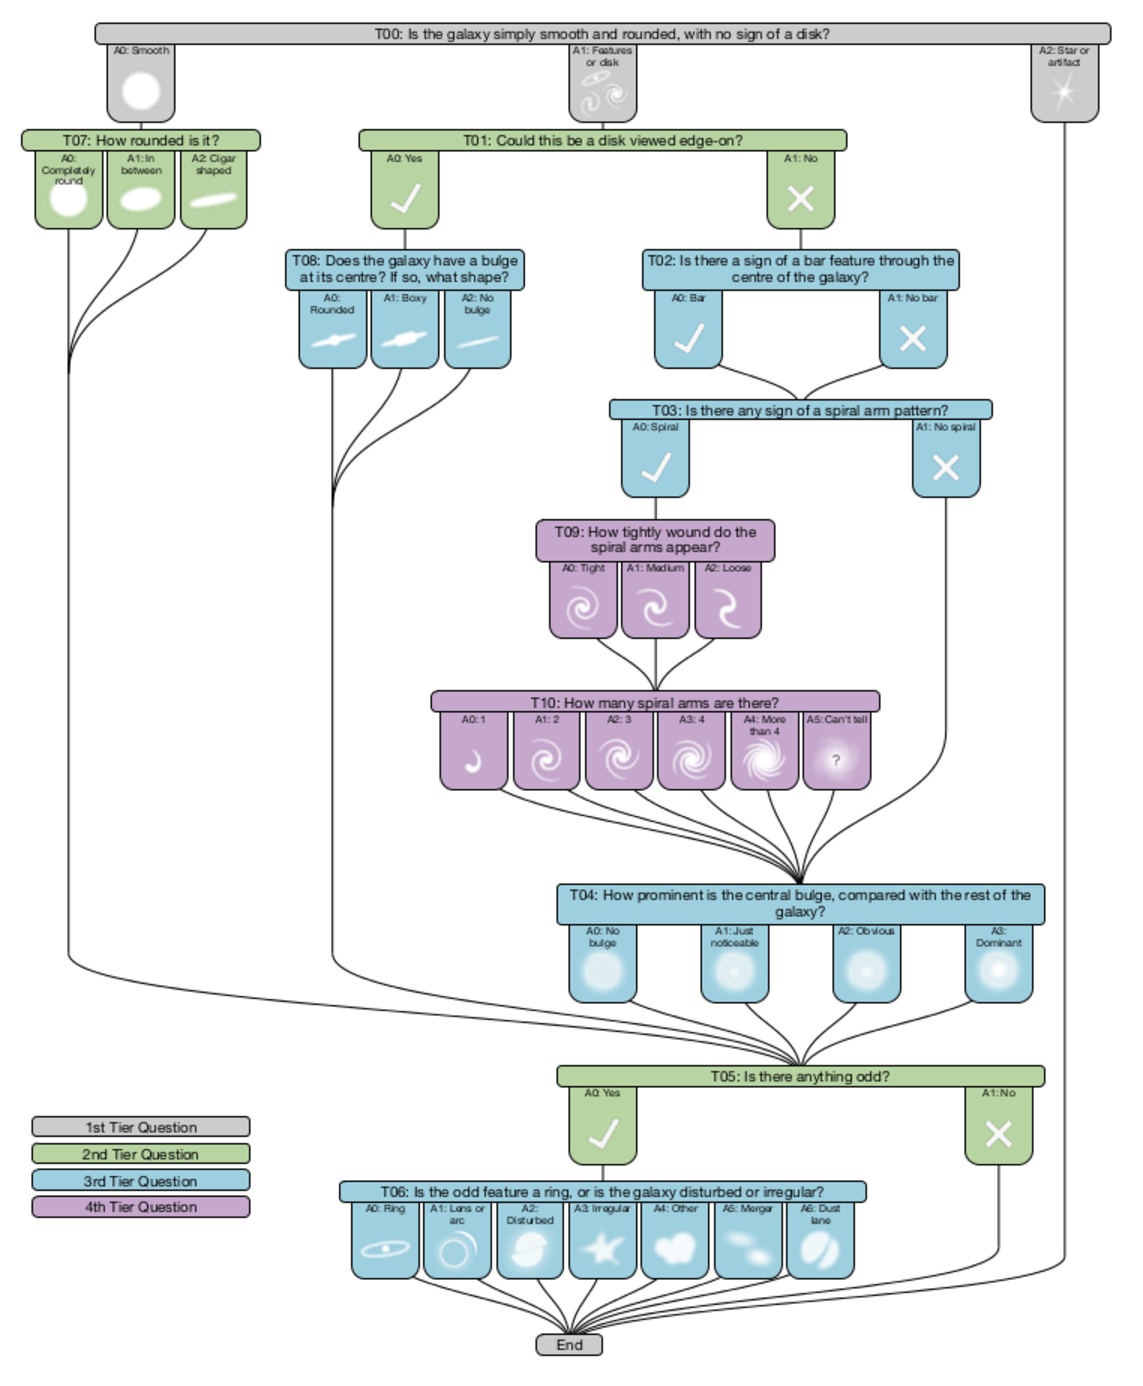
\includegraphics[width=\textwidth]{Figures/gz2_tree.pdf}
\caption[Galaxy Zoo 2 decision tree]{Galaxy Zoo 2 decision tree structure.}
\label{fig: gz2 decision tree}
\end{figure}

For the single-depth sample, volunteers were shown color images generated from the SDSS ImgCutout web service. Each image is a $gri$ color composite scaled to $0.02\times$\texttt{petror90\_r}. Throughout the life of GZ2 these images were randomly served to a web interface similar to that shown in Figure \ref{fig: gz2 interface}. Towards the end of the project galaxy images with few responses were shown more frequently in order to ensure that each galaxy had a sufficient number of classifications to adequately characterize the likelihood of the classification distribution. This resulted in a median of 44 classifications per galaxy with a wide spread. The full project spanned just over 14 months with the final dataset consisting of over 16 million classifications from over 80 thousand volunteers. 
 
%%%%%%%%%%%%%%%%%%%%%%%%%%%%%%%%%%%%%%%%%%%%%%%%%%%%%%%%%%%%%%%%%%%%%%%%%%
%%%		FIGURE: 	GZ2 WEB INTERFACE
%%%%%%%%%%%%%%%%%%%%%%%%%%%%%%%%%%%%%%%%%%%%%%%%%%%%%%%%%%%%%%%%%%%%%%%%%%
\begin{figure}[h!]
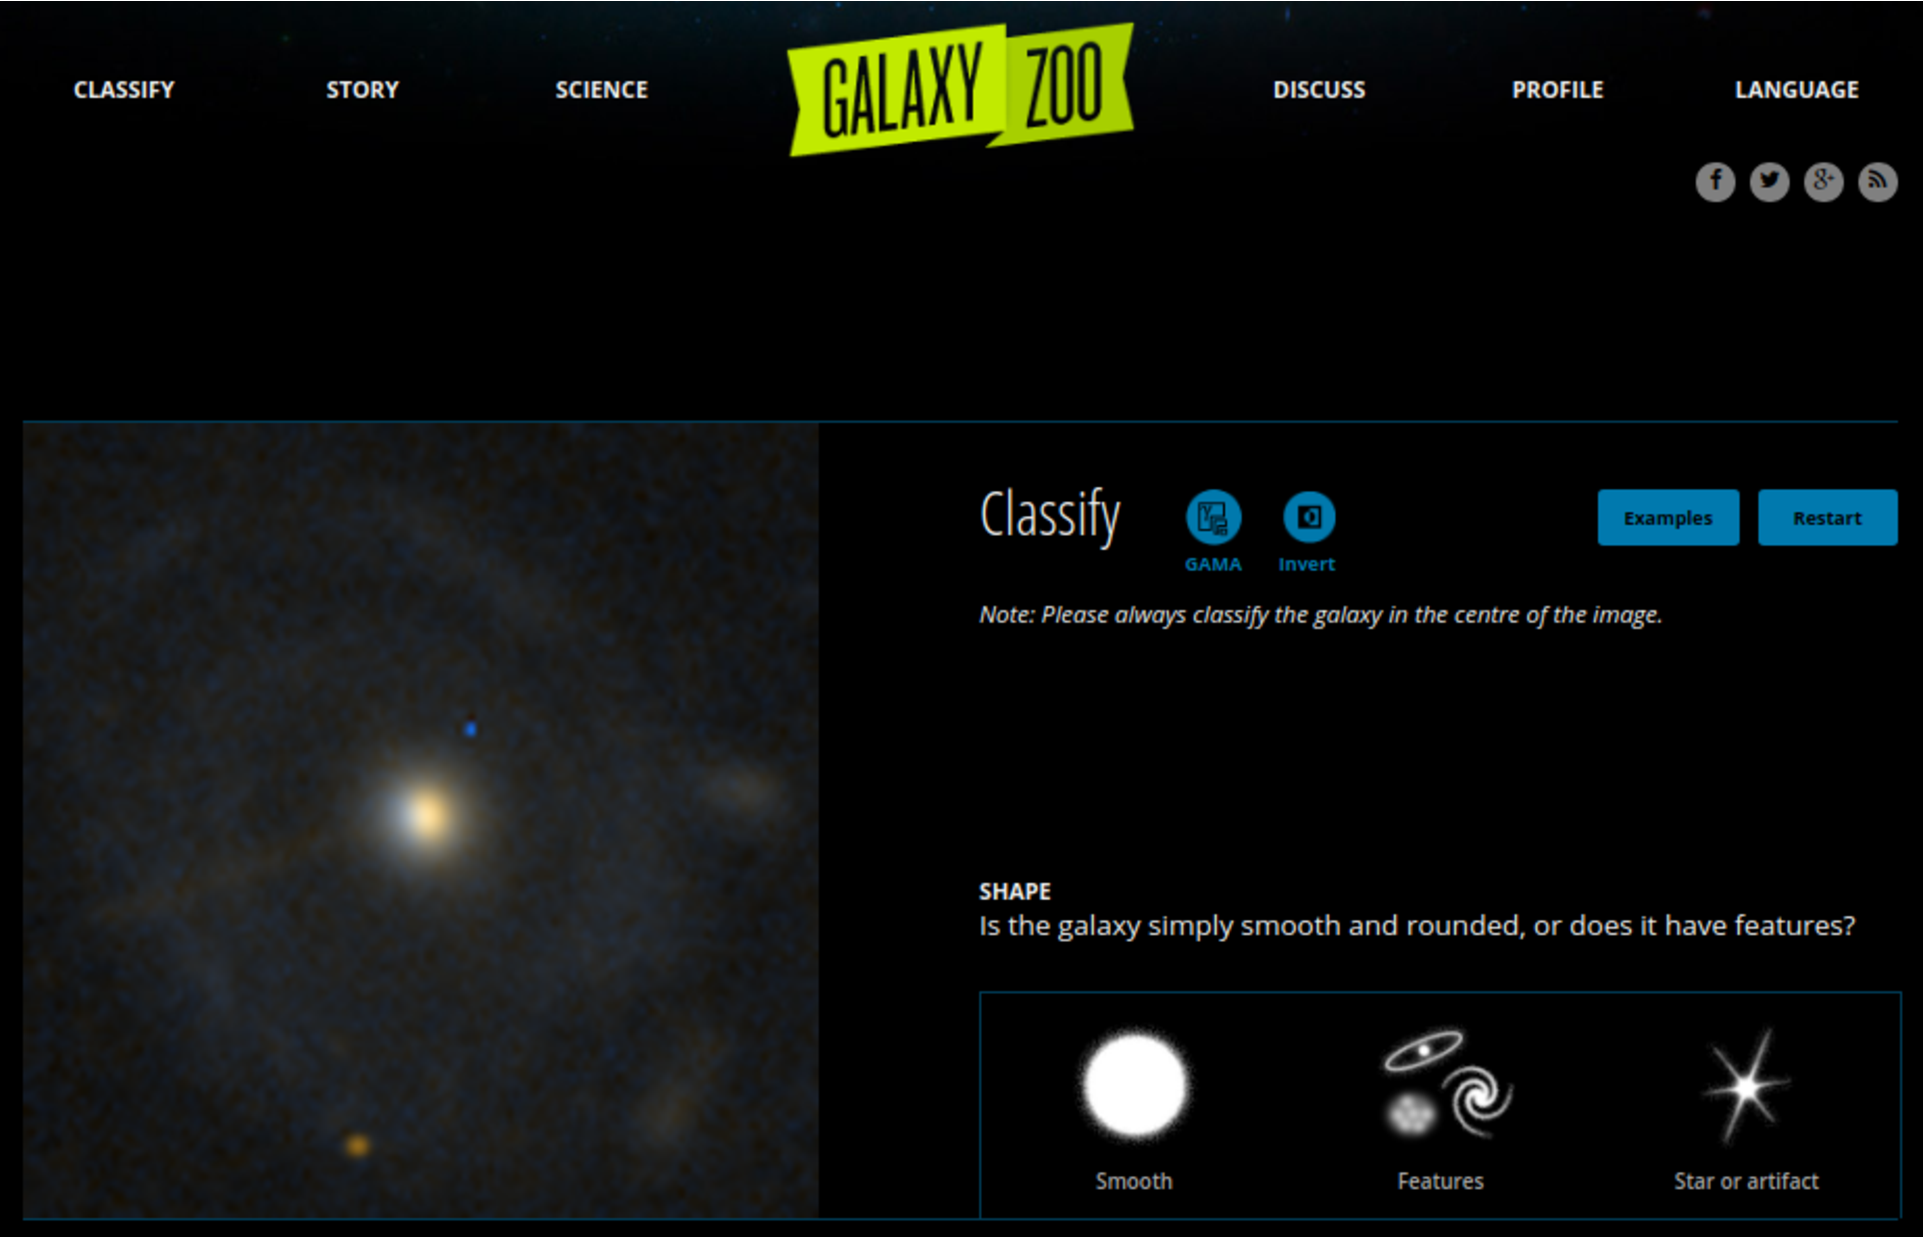
\includegraphics[width=\textwidth]{Figures/GZ2interface.pdf}
\caption[Example of the Galaxy Zoo 2 web interface]{Example of the Galaxy Zoo 2 web interface showing the first question in the decision tree.}
\label{fig: gz2 interface}
\end{figure}

%%%%%%%%%%%%%%%%%%%%%%%%%%%%%%%%%%%%%%%%%%%%%%%%%%%%%%%%%%%%%%%%%%%%%%%%%%
%%%		SUBSECTION: 	DATA REDUCTION
%%%%%%%%%%%%%%%%%%%%%%%%%%%%%%%%%%%%%%%%%%%%%%%%%%%%%%%%%%%%%%%%%%%%%%%%%%
\subsection{Data reduction}
The GZ2 catalog provides several types of morphologies computed from volunteer classifications constisting of a vote fraction for each response to every task, denoted $f_{\mathrm{response}}$. The most basic of these is computed simply as $f_r = n_r/n_t$, where $n_r$ is the number of votes of response $r$, and $n_t$ is the total number of votes for task $t$. In future chapters, this type of vote fraction is referred to as the \textit{raw} vote fraction as no post-processing has been performed. 

All GZ projects perform a weighting scheme that evaluates the consistency of individual volunteers by assessing how their votes deviate from the majority for each task in the decision tree. This process effectively downweights volunteers whose responses are consistent with a random classifier. A volunteer's consistency, $\kappa$, for a given task is defined as 

\begin{equation}
\kappa = \frac{1}{N_r}\sum_{i=1}^{N_r}{\kappa_i}
\end{equation}
where $N_r$ is the total number of responses to a task, and $\kappa_i$ is $f_r$ if the volunteer's vote corresponds to response $i$, otherwise $\kappa=(1-f_r)$. Each volunteer is then assigned a mean consistency, $\bar\kappa$, which is the average consistency over all tasks. A weighting function is then applied according to  

\begin{equation}
w = \min({1.0, (\bar\kappa/0.6)^{8.5}}).
\end{equation}

All vote fractions are then recomputed using the volunteer weights and the process is repeated three times to assure convergence. The resulting vote fractions are dubbed \textit{weighted}. For GZ2, $w=1$ for $\sim$95\% of volunteers and thus the majority are treated equally. It's important to note that there is no up-weighting of exceptionally consistent volunteers.


Finally, when considering morphologies, be they visual or automatic, for a sample of galaxies in a small redshift range it is unlikely that galaxy evolution plays a major role in morphology variations. Thus, the presumed culprit is instead classification bias in that galaxies in the more distant universe tend to be, on average, smaller and dimmer. This obscures identification of features such as spiral arms, bars, and more. GZ2 corrects for this effect, briefly described below, producing \textit{debiased} vote fractions.

The general approach is such that, for a galaxy of a given size and brightness, a sample of other galaxies with similar characteristics will statistically share the same mix of morphologies. Thus the GZ2 main galaxy sample is binned by Petrosian absolute magnitude (M$_r$) and the Petrosian half-light radius, R$_{50}$,  as well as by redshift. A baseline morphology ratio is computed in the lowest redshift bin for those galaxies in the same with confirmed spectroscopic redshifts and with sufficient numbers of votes to yield statistically reliable classifications. This basiline is then used to correct more distant redshift bins. A more detailed account can be found in \cite{Willett2013}.

%This thesis draws on the \textit{raw} vote fractions for reasons explained in Chapter \ref{chap:3}. Focus now turns to the methodology of measuring automatic morphological indictors which are used in Chapter \ref{chap:4} to train a machine classifier. 

%%%%%%%%%%%%%%%%%%%%%%%%%%%%%%%%%%%%%%%%%%%%%%%%%%%%%%%%%%%%%%%%%%%%%%%%%%
%%%		SECTION: 	AUTOMATIC MORPHOLOGY INDICATORS
%%%%%%%%%%%%%%%%%%%%%%%%%%%%%%%%%%%%%%%%%%%%%%%%%%%%%%%%%%%%%%%%%%%%%%%%%%
\section{Automatic morphology indicators}
This thesis seeks to draw on the best qualities of all galaxy morphology classification methods including using automated morphologies and machine learning algorithms which provide speed and brute force. Any machine classifier must have a set of features from which to learn to differentiate between classes. These features can be anything that correlates or distinguishes among class labels. In the case of galaxy morphology possible features could include pixel values, spectral indices, magnitude, color, etc. Choosing which features are most appropriate for each task is a difficult task as there are no clear cut rules for feature selection. Too few features and a machine learning algorithm will be unable to learn the parameter space; too many features can result in the Curse of Dimensionality: as the dimensionality of the parameter space increases linearly, the number of samples required to learn that space increases exponetially! 

In this work we draw on the Zurich Estimator of Structural Types \citep[ZEST,][]{Scarlata2007}. ZEST utilized five features measured from the light profile of galaxy images combined with a PCA analaysis to determine morphologies for 120K COSMOS galaxies. These features are well known to correlate strongly with the distinction between early- and late-type galaxies. In this section we discuss how these values are measured for the GZ2 SDSS galaxy sample. 

\subsection{Imaging data}
The Galaxy Zoo 2 main galaxy sample contained 295,305 galaxies though 11,334 are single-epoch imaging from the Stripe 82 region with m$_r > 17.0$, fainter than the rest of the galaxy sample. These galaxies are excluded from the main GZ2 classification catalog though classifications for these galaxies exist in Stripe 82-exclusive catalogs. However, because we utilize the raw volunteer classifications from the original GZ2 project, we include all single-epoch galaxy imaging in our current sample, regardless of magnitude limit.  

We obtain $i$-band imaging (with central wavelength 7480\AA) from SDSS Data Release 12 for 290,059 galaxies in the GZ2 project. Image identifier such as \texttt{CAMCOL}, \texttt{RUN}, and \texttt{FIELD} are used to select over 151,987 SDSS fields. Because the original GZ2 project obtained imaging from DR7, we surmise that the route to some galaxies in DR12 have switched locations or identifiers thus explaining the loss of 5246 galaxies. Because this represents only 1.8\% of the total population, these galaxies were not tracked down at this time. Postage stamps of each galaxy are cut from these fields where the dimensions of each cutout are 4$\times$Petrosian radius as measured by the SDSS pipeline. Galaxies located within 4 Petrosian radii of the edge of a field were excluded as image mosaicing was not performed. This removed 7962 galaxies resulting in a final sample of 282,350 GZ2 galaxy postage stamps or 95.6\% of the original sample.

\begin{figure}
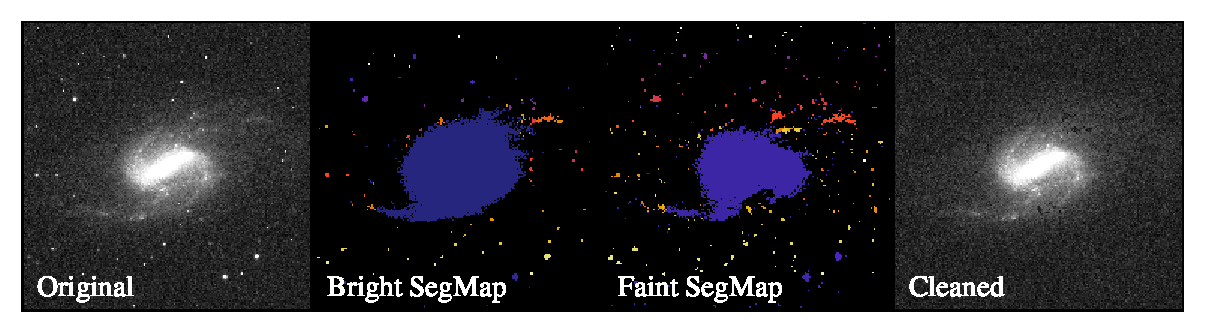
\includegraphics[width=\textwidth]{Figures/sextractor_example.pdf}
\caption[Example of Source Extractor segmentation maps.]{Example of SExtractor segmentation maps generated during the postage stamp cleaning process. The left panel shows the original $i$-band postage stamp, the middle two panels show the bright and faint segmentation maps where individual objects detected by SExtractor are shown on an arbitrary rainbow scale, and the right panel shows the resulting cleaned postage stamp.}
\label{fig: segmaps}
\end{figure}


\subsection{Image cleaning}
These postage stamps next undergo a cleaning process in order to remove the light from nearby sources so as not to contaminate the light profile of the galaxy of interest. Each stamp is processed through Source Extractor \citep[ver. 2.8.6;][]{sextractor}, a software that automatically detects sources in CCD imaging based on a set of input parameters that control its sensitivity. Two sets of parameters are used: the first is designed to identify bright sources, while the second is better optimized to detect fainter objects. This software produces segmentation maps that identify the boundaries of each detected object in an image. By design, the galaxy of interest is located at the center of the cutout. Extraneous sources are then identifed from both the bright and faint segmentation maps and the pixels corresponding to these sources are replaced with a random value consistent with the background in that postage stamp.  An example of the segmentation maps created during this process is shown in Figure \ref{fig: segmaps}. Additionally, the first two columns in \Cref{fig: morph examples,fig: morph examples 2,fig: morph examples hardest} depict random samples of original and cleaned cutouts for a variety of ``difficulties,'' where the difficulty of successfully cleaning an image of all stray light from other nearby sources is dependent upon how many other sources exist in the postage stamp and how close those sources are to the galaxy of interest. 


\begin{figure}
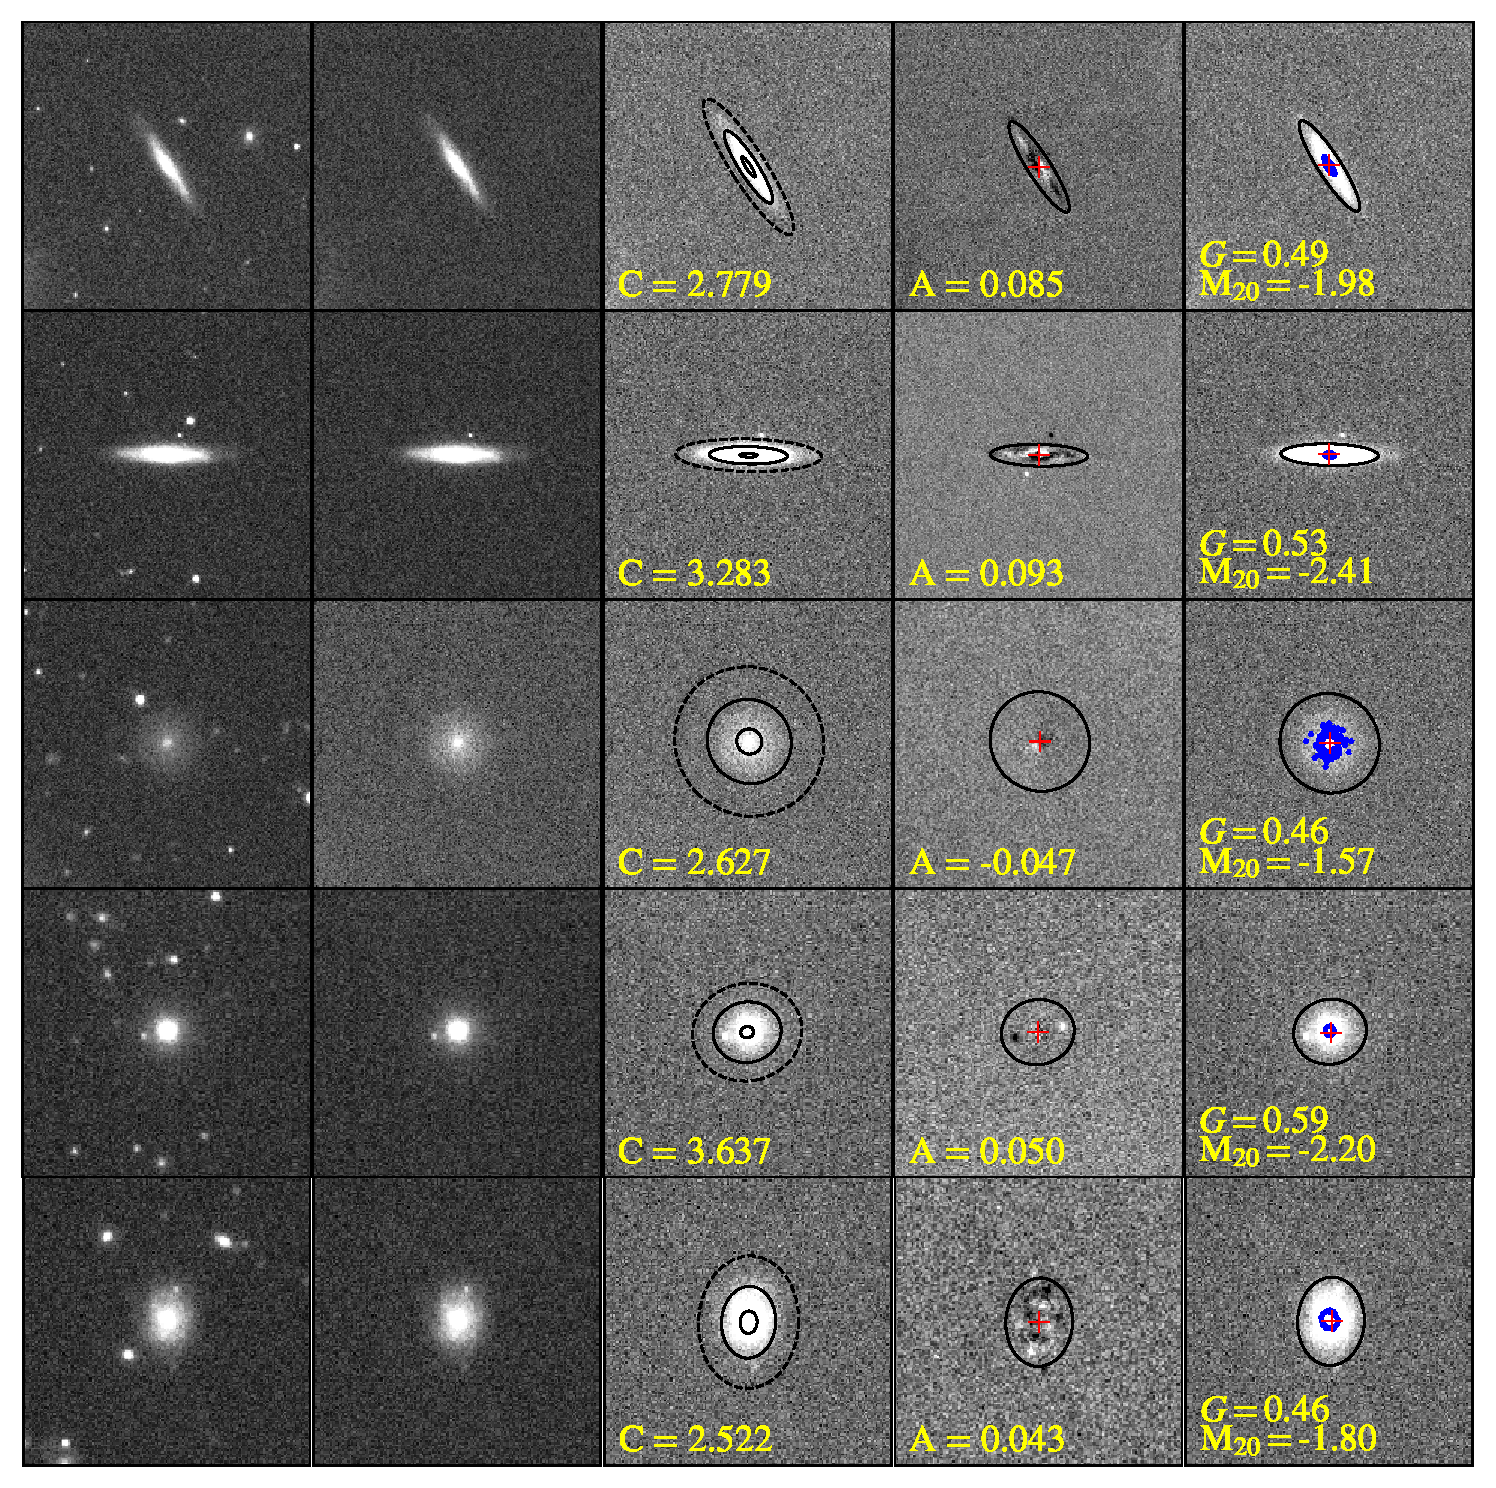
\includegraphics[width=\textwidth]{Figures/measure_morph_bin2_corrected.pdf}
\caption[Examples of image cleaning and morphology diagnostic measurements]{Examples of the postage stamp cleaning and morphology diagnostic measuring processes. The first and second columns show the original and cleaned $i$-band postage stamps. The third column shows the apertures used to calculate the concentration index where the two solid ellipses represent the apertures enclosing 20\% and 80\% of the galaxy total light which is defined as 1.5$\times$\rp~and shown as a dashed ellipse. The fourth column shows the residual asymmetry image generated according to Equation \ref{eqn: asymmetry} where the red cross denotes the galaxy's asymmetry center. The final column shows the Gini and \M{20} values where the red cross denotes the galaxy's \M{20} center and the blue contours trace the brightest 20\% of galaxy pixels. In the two rightmost columns, the solid ellipse represents 1\rp~within which all morphology diagnostics are computed.}
\label{fig: morph examples} 
\end{figure}


\begin{figure}
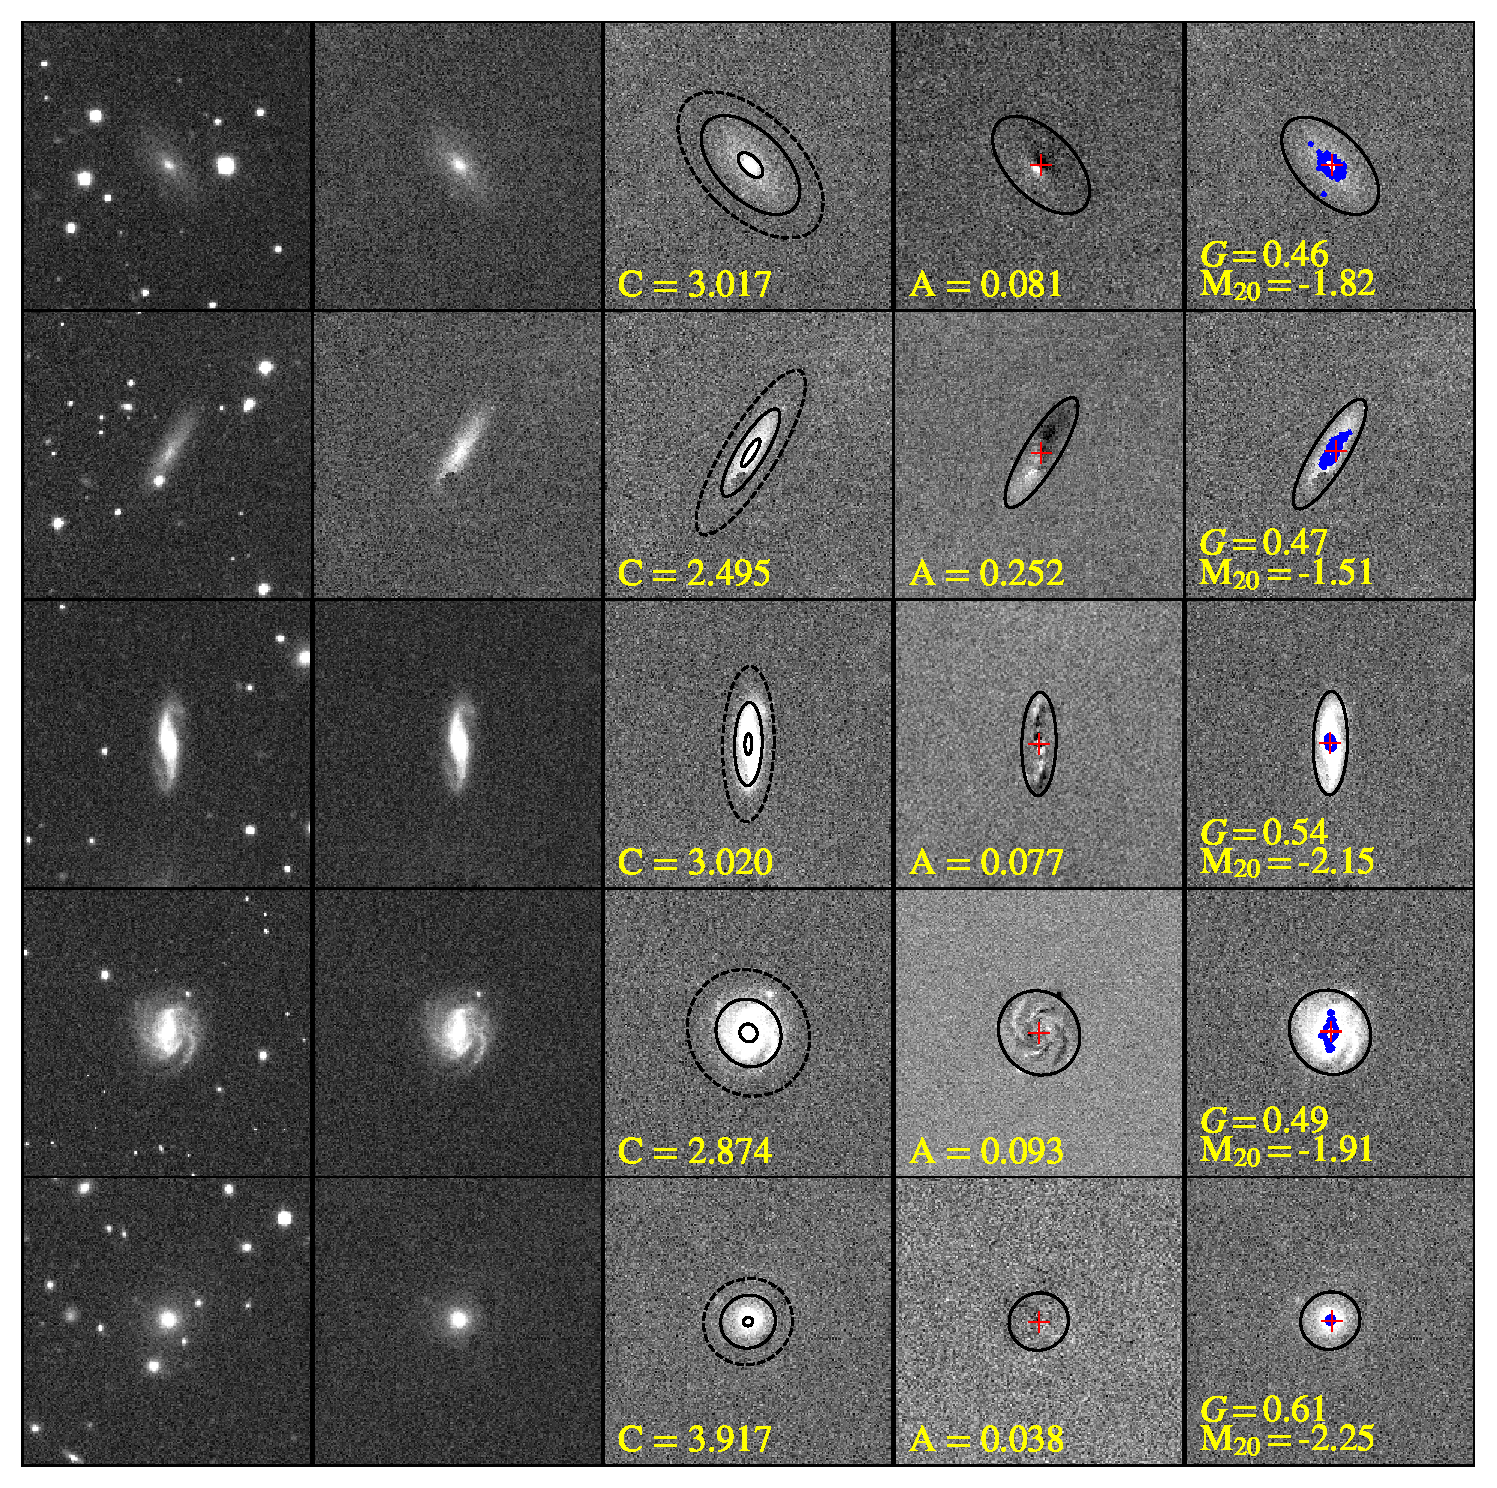
\includegraphics[width=\textwidth]{Figures/measure_morph_bin3_corrected.pdf}
\caption[Examples of image cleaning and morphology diagnostic measurements]{Additional examples of the postage stamp cleaning and morphology diagnostic measuring processes. See caption from Figure \ref{fig: morph examples}.}
\label{fig: morph examples 2}
\end{figure}

\begin{figure}
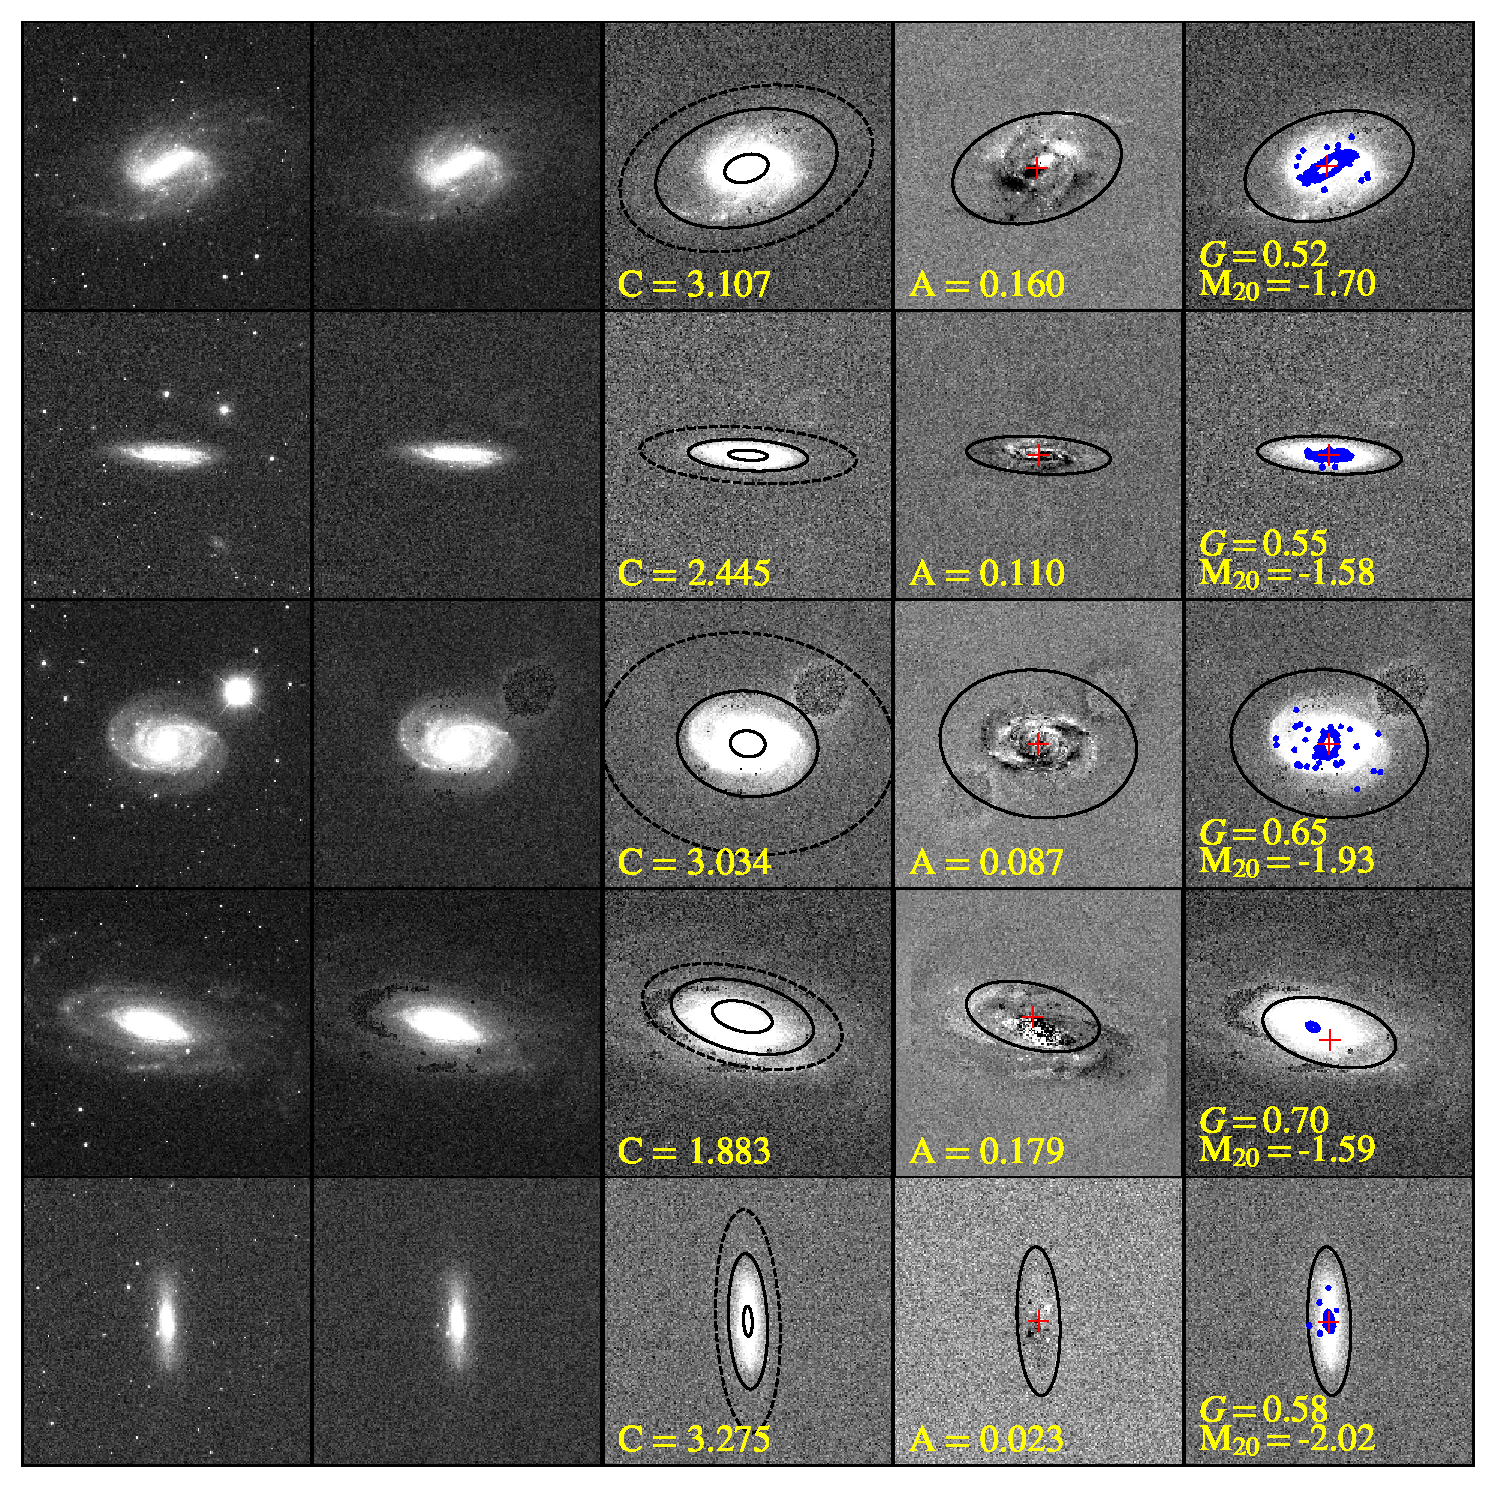
\includegraphics[width=\textwidth]{Figures/measure_morph_hardest.pdf}
\caption[Examples of image cleaning and morphology diagnostic measurements]{Examples of the postage stamp cleaning and morphology diagnostic measuring processes for a random sample of the largest and most difficult galaxies. See caption from Figure \ref{fig: morph examples}.}
\label{fig: morph examples hardest}
\end{figure}


\subsection{Morphology indicators}
Defining the flux associated with a galaxy is a challenging task: galaxies do not have constant radial surface brightness, hard edges, or uniform shapes.  One way to measure the flux is to consider the light within some isophote but the fraction of light included within will be dependent on the amplitude of the galaxy's surface brightness which diminishes due to cosmological redshift and Galactic extinction. To combat these issues, it is common practice to use the \cite{Petrosian1976} system which computes a radius defined by the empirical shape of the galaxy's light profile. Specifically, the Petrosian radius, \rp, is such that the ratio of the surface brightness at \rp~to the mean surface brightness within \rp~is equal to a fixed value $\eta$, i.e., 
%Ideally, one would measure the total flux associated with a galaxy but this requires modelling of the light profile in addition to high signal-to-noise ratio in the outermost parts of the galaxy.

\begin{equation}\label{fig: petrosian raidus}
\eta = \frac{\mu(r_p)}{\bar\mu(r<r_p)}
\end{equation}
where $\eta$ is traditionally set to 0.2. Because this is a ratio of surface brightnesses, cosmological factors are mitigated. 

We compute \rp~by first generating a set of elliptical annuli centered on the galaxy and equidistant in logspace. At least 20 annuli are used for each postage stamp. Elliptical apertures minimize the contribution from noisy background pixels. The position angle and galaxy center are taken from the SExtractor catalogs generated ealier. For each annulus, $\mu(r_i)$ is computed as the flux within the annulus divided by the annulus area, while $\mu(r<r_i)$ is computed as the total flux integrated to the center of that annulus divided by $\pi r_i^2$. This provides a crude estimate of $\eta$ which is then interpolated onto a finer set of radial values.  \rp~is that radius for which $\eta$ intersects 0.2. Examples of surface brightness profile are shown in Figure XXX. XX demonstrates a case in which the cleaning algorithm did not fully remove nearby contaminating light from other sources, resulting in an $\eta$ that never crosses the 0.2 threshold. To correct for this, we model the excess light in the outer component with a linear relation and subtract a constant value from the surface brightness profile. Even with these measures, some failures persist, however, we are only unable to obtain \rp~for 16 galaxies, a vanishingly small fraction of our sample. We use these values of the Petrosian radius to compute the following morphology diagnostics.


%\subsubsection{Concentration}
Concentration is defined in several slightly different ways with the aim being to measure the ratio of the light within an inner aperture to that within an outer aperture. Small values of this ratio typically indicate disky galaxies, while larger values correlate with early-type ellipticals. We use the definition of \cite{Bershady2000}:

\begin{equation}\label{eqn: concentration}
C = 5\log\Big(\frac{r_{80}}{r_{20}}\Big) 
\end{equation}
where \rr{80} and \rr{20} are the radii containing 80\% and 20\% of the total galaxy light respectively where we define the total flux as that within \rp~and the galaxy center is that determined by the asymmetry minimization \cite[described below,][]{Lotz2004}. A random sample of concentration measurements can be seen in the middle column of \Cref{fig: morph examples,fig: morph examples 2,fig: morph examples hardest}. 

The asymmetry parameter, $A$, quantifies the degree of rotational symmetry in the galaxy light distribution, not necessarily the physical shape of the galaxy as this is not highly sensitive to low surface brightness features. $A$ is measured by subtracting the galaxy image rotated by 180$^{\circ}$. A correction for background noise is applied \citep[as in e.g.,][]{Conselice2000, Lotz2004}, i.e., 
\begin{equation}\label{eqn: asymmetry}
A = \frac{\sum_{x,y} |I(i,j) - I_{180}(i,j)|}{ 2\sum|I(i,j)|} - B_{180}
\end{equation}
where $I$ is the galaxy flux in each pixel $(x, y)$, $I_{180}$ is the image rotated by 180 degrees about the galaxy's central pixel, and $B_{180}$ is the average asymmetry of the background. $A$ is summed over all pixels within \rp~of the galaxy's center and then normalized by a corresponding measure in the original image. The center is determined by minimizing $A$ as described in \cite{Conselice2000}. Briefly, an initial central pixel is chosen and $A$ computed. Then asymmetry is calculated again in a $3\times3$ grid about that central pixel. If one of these produces a lower value of $A$, it becomes the new center and the process repeats until a minimum is found. This is a crucial step as \cite{Conselice2000} find that a small difference can change the asymmetry by up to 50\%. Additionally, the effects due to noise must also be corrected. This is accomplished by selecting a blank portion of the cutout with the same pixel area as defined for the $A$ measurement.  $A$ is computed as before, including the minimization, and this value then constitutes $B_{180}$. A random sample displaying the apertures and asymmetry centers are shown in the fourth columns of\Cref{fig: morph examples,fig: morph examples 2,fig: morph examples hardest}. 

The Gini coefficient, $G$, has long been used in econometrics as a measure of inequality by estimating the concentration of wealth in a nation's population. It is based on the Lorenz curve \citep{Lorenz1905} which is constructed by mapping the cumulative proportion of the population ranked by wealth onto the corresponding cumulative proportion of the size of their wealth. More formally, if $X$ is a positive random variable with cumulative distribution function $F(x)$ then the Lorenz curve goes as   
\begin{equation}
L(p) = \frac{1}{\bar X}\int^p_0 F^{-1}(u)~du,
\end{equation}
where $p$ is the percentile of the poorest denizens, and $\bar X$ is the mean over all values of $X_i$, a random deviate drawn from $X$. $G$ is then a summary statistic of this curve describing the mean of the absolute difference between all combinations of $X_i$:

\begin{equation}
G = \frac{1}{2\bar Xn(n-1)}\sum_{i=1}^n\sum_{j=1}^n\Big|X_i - X_j\Big|.
\end{equation}
This statistic was first applied to the distribution of a galaxy's light by \cite{Abraham2003} and further developed by \cite{Lotz2004}. In these terms, $G$ is 0 when the galaxy's flux is distributed homogeneously among all assigned pixels, and 1 if the light is concentrated within a single pixel. $G$ can be calculated more efficiently if the $X_i$ are first sorted into increasing order and then computing \citep{Glasser1962}
\begin{equation}
G = \frac{1}{|\bar X|n(n-1)}\sum_i^n(2i-n-1)|X_i|,
\end{equation}
where $n$ is the number of pixels assigned to the galaxy. Here we follow \cite{Lotz2004} by taking the absolute value of the flux, $X_i$, because in pixels with low signal-to-noise the flux is scattered to values below the mean sky level resulting in negative flux values for the faintest pixels. 

Assigning pixels to each galaxy must be given due consideration. As \cite{Lotz2004} point out, including too many sky pixels will systematically increase $G$, while exclusion of low surface brightness galaxy pixels will decrease $G$. \cite{Abraham2003} measure $G$ for pixels above a given surface brightness threshold but this will fall prey to cosmological effects. In this work, we compute $G$ from all pixels within \rp. This will exclude some low surface brightness features, especially for galaxies with faint, extended elements. However, this definition puts every galaxy on equal footing, and as we discuss in Chapter \ref{chap:4}, systematics are easily handled by the machine learning algorithm we exploit. The last column in \Cref{fig: morph examples,fig: morph examples 2,fig: morph examples hardest} shows examples of $G$.

%\subsubsection{M$_{20}$}
\M{20}~\citep{Lotz2004} is the second order moment of the brightest 20\% of the galaxy flux. It traces the spacial distribution of any bright galactic features such as nuclei, bars, spiral arms, or star-forming clusters. It is computed by first calculating the total moment as
\begin{equation}
 M_{\mathrm{tot}} = \sum_i^n M_i = \sum_i^nf_i[(x_i-x_c)^2 + (y_i-y_c)^2] 
\end{equation}
where $f_i$ is the flux in pixel $x_i$, $y_i$, and $x_c$, $y_c$ is the galaxy's center which is determined by minimizing $M_{tot}$ in a similar fashion as is done for the asymmetry. The galaxy pixels are then ranked by flux in descending order and $M_i$ is summed over the brightest pixels until that sum equals 20\% of the total galaxy flux, normalized by $M_{\mathrm{tot}}$:
\begin{equation}
 M_{20} = \log_{10} \Big( \frac{\sum_iM_i}{M_{\mathrm{tot}}} \Big), ~~\textrm{while} \sum_if_i < 0.2f_{\mathrm{tot}}
\end{equation}
where $f_{tot}$ is the total flux defined within \rp. For centrally concentrated objects, \M{20} correlates with $C$ but is also sensitive to bright off-centre knots of light. 

It's worth noting that both \M{20} and $G$ are correlated with $C$, but with key differences. Because $G$ is a measure of concentration it correlates strongly with $C$, especially for local galaxies \cite{Abraham2003}. However, $G$ is independent of spatial distribution: whereas $C$ measures the concentration in the central region of a galaxy, $G$ is sensitive to any concentration of light: centralized or not. M$_{20}$ takes this a step further with its key difference being a strong $r^2$ dependence. It is strongly weighted by the spatial distribution of bright regions but these need not be centralized either.  Indeed, when $G$ and \M{20} are taken together they are highly adept at identifying merging galaxies \citep{Lotz2004,Lotz2008}.  


%\subsubsection{Ellipticity}
For our final morphology diagnostic, we use the ellipticity, $\epsilon = 1 - b/a$, of the light distribution as measured by SExtractor which computes the semi-major axis $a$ and semi-minor axis $b$ from the second-order moments of the galaxy light. The ellipticity of a galaxy correlates strongly with edge-on galaxies. 

In total, we measure morphological indicators for 282,350 SDSS galaxies. Some galaxies are lost at each stage of the measurement process due to various failures which we discuss in detail below. For example, if our measurement of the Petrosian radius is not successful, no morphology diagnostics are computed for that galaxy. The number of galaxies with successful measuremenets at each stage is listed in Table \ref{tab:morph numbers}.  The relations between these diagnostics for the full sample is shown in Figure~\ref{fig: morph thresh}. The code developed to clean and compute these morphology indicators is open source and can be found at \url{https://github.com/melaniebeck/measure_morphology}.

% From the Selecting Random Subsamples for Thesis Chap3 (jupyter notebook)
\begin{table*}[]
	\centering
	\caption[Summary of morphology measurements (UPDATE THIS)]{}
	\label{tab:morph numbers}
	\let\mc\multicolumn
	\begin{tabular}{lccc}
		\mc4c{ \textbf{Morphology measurement summary}} \\
		\hline \hline
			&	&	&	\\
								  & Number &  \% Success & Notes \\
		\hline
		Full Galaxy Zoo 2 sample  	& 295 305 &	   &  \\
		Postage stamps 				& 282 350 &		95.6 	&  \% of full sample\\
		Petrosian radius			& 282 334 &		99.99 	& \% of postage stamps\\
		Concentration				& 281 927 &		99.85 	& \% of postage stamps\\ 	
		Asymmetry 					& 282 334 &		99.99 	& \% of postage stamps\\
		Gini coefficient			& 282 323 &		99.99	& \% of postage stamps\\
		M$_{20}$					& 282 194 &		99.94 	& \% of postage stamps\\	
		Ellipticity ($1 - b/a$)		& 282 350 &		100.0 	& \% of postage stamps\\
		\hline
	\end{tabular}
\end{table*}

\subsection{Quality and consistency}
We perform several checks to determine the quality and consistency of our morphology diagnostics. Due to the wealth of information provided by the SDSS pipeline, we can compare some of our diagnostics against SDSS values. Obviously there are some instances where our measurements will outperform the SDSS pipeline and vice versa. We first check our values of the Petrosian radius as shown in Figure \ref{fig: Rp comparison}. Our \rp~are on average $\sim$35\% larger than those computed by SDSS. The biggest reason for this discrepancy is due to aperture shape: SDSS compute \rp~using circular annuli while we use elliptical. [Mention the weird ones where our \rp~is tiny but SDSS's is huge? Show some examples where my code does better than SDSS? And where mine fails?]

\begin{figure}
\centering
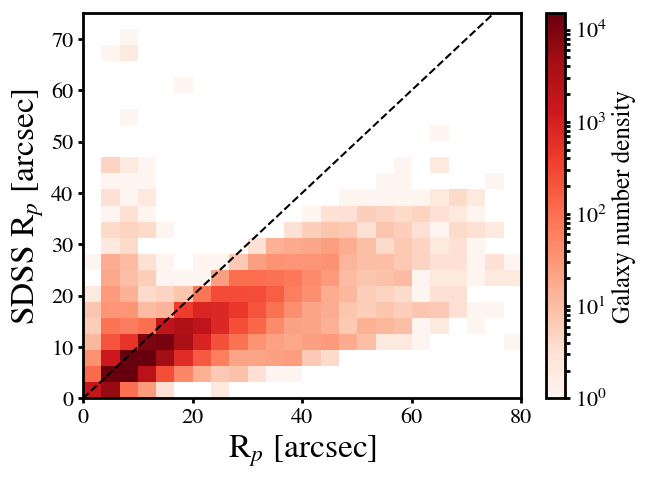
\includegraphics[width=5in]{Figures/PetroRad_compare_cleanSample_forThesis.png}
\caption[Comparison of Petrosian radius from this work to that computed in SDSS pipeline]{Comparison of the Petrosian radius R$_p$ computed in the SDSS pipeline to that caluclated in this work. Most of the discrepancy between these values is due to the apertures used: the SDSS pipeline defines R$_p$ in circular annuli while we use elliptical.}
\label{fig: Rp comparison}
\end{figure}

Of greater importance, however, are the values of the morphology diagnostics as these are used as features to train our machine learning algorithm in Chapter \ref{chap:4}. Though SDSS does not measure all of the structural indicators we tackle here, they do provide a means to compute the concentration index via \texttt{PETROR50} and \texttt{PETROR90}, the Petrosian radii containing 50\% and 90\% of the galaxy total light, respectively. The left panel of Figure \ref{fig: concentrations}~shows our $C$ against that computed from SDSS, $C_{\mathrm{SDSS}}$. Our values are systematically $\sim$1 point larger than SDSS values but otherwise retain a strikingly tight correlation. This is suprising considering the drasticly different ways these values are computed. Besides the obvious difference in radii (SDSS uses 50\% and 90\% vs our 20\% and 80\%), SDSS values are again computed using ciruclar apertures whereas we use elliptical for all measurements. The latter are preferable as it has been shown that aperture shape affects $C$ \citep{Bershady2000, Andrae2011}. This is hinted at in the right panel of Figure \ref{fig: concentrations} which shows the ratio $C$/$C_{\mathrm{SDSS}}$ as a function of galaxy elongation. \cite{Andrae2011} demonstrate a bias such that the concentration index is artificially inflated when measured from circular apertures for highly elongated galaxies. Instead the opposite should be seen, that is, early-type galaxies tend to have much higher concentrations and are generally less elongated (compared to edge-on disks!). This is the trend we see in the right panel due to the fact that we use elliptical apertures to compute $C$ and thus our $C$ values are less prone to this potential bias.


\begin{figure}
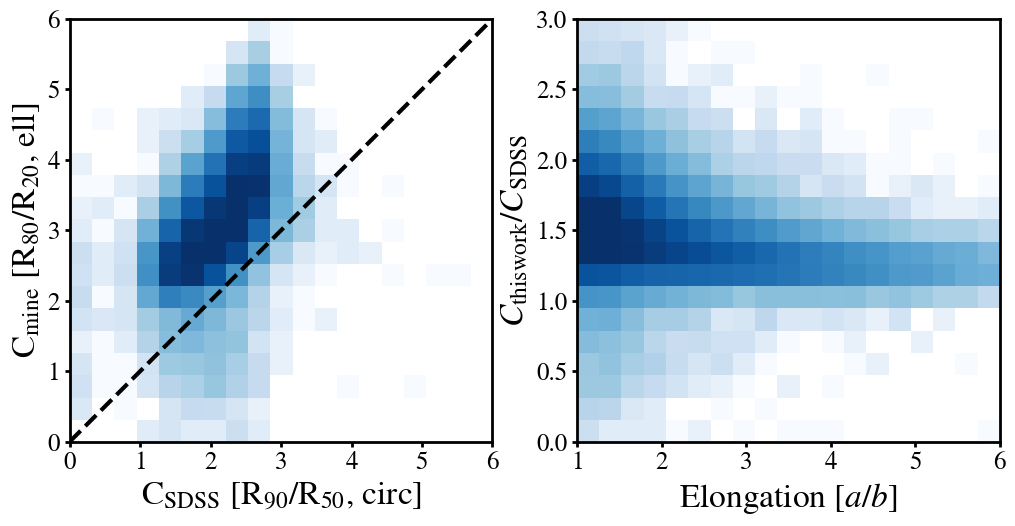
\includegraphics[width=\textwidth]{Figures/compare_concentrations.png}
\caption[Comparison of concentration index from this work to that computed from SDSS.]{The left panel shows our measured concentration index against that computed from values taken from SDSS DR7. We find that our $C$ is systematicaly $\sim$1 point larger than SDSS. This is quite remarkable considering $C_{\mathrm{SDSS}}$ is computed using Petrosian radii containing 50\% and 90\% of the total galaxy light, while we use radii containing 20\% and 80\% of the galaxy total light. Additionally, SDSS use circular annuli when computing their radii whereas we use elliptical. The right panel shows the ratio $C$/$C_{\mathrm{SDSS}}$ as a function of galaxy elongation. }
\label{fig: concentrations}
\end{figure}


SDSS does not provide any other direct morphology diagnostics comparable to what we measure here so we next assess the quality of our structural indicators by estimating the fraction that are poorly measured. We consider the galaxy central coordinates assigned at various stages during the cleaning and measuring process and compare those to the original SDSS galaxy coordinates. SExtractor assigns galaxy central coordinates for each postage stamp based on the first order moment of light. Additionally, the asymmetry and \M{20}~measurements each determine their own galaxy center via the minimization of their respective quantity and thus do not necessarily overlap. We compute the coordinate difference in arcseconds for each of these three centers as compared to the SDSS coordinates and determine that only 3.0\%, 1.9\%, and 1.5\% of galaxies have SExtractor, asymmetry and \M{20} centers, respectively, that differ by more than $1\arcsec$ from the original SDSS coordinates. Thus we find very good agreement between SDSS and SExtractor galaxy centers, indicating that we correctly identify the galaxy of interest in each postage stamp. We also find good agreement between SDSS and both the $A$ and \M{20} centers indicating that our minimizing algorithm fails only in a handful of instances.  

%Though all of these morphological diagnostics are subject to resolution, signal-to-noise, and aperture size and shape variability, the Gini coefficient is arguably the most susceptible to such issues \citep{Lisker2008}. 

Finally we consider the overall distribution of our measured structural indicators. It is well known that different galaxy types live in different parts of morphology parameter space. For example, in the $G$-\M{20} plane, early-type galaxies are typically found in the upper right with late-type galaxies residing in the lower left, and merging systems in the upper left. Similar relations exist in the $C$-$G$, and $G$-\M{20}~planes. In Figure \ref{fig: morphs as a fcn of fsmooth}~we select a random sample of 5000 galaxies and plot them in each possible planar combination of our morphology diagnostics where the points are colored according to their Galaxy Zoo 2 debiased \fsmooth~fraction. Because \fsmooth~correlates well with early-type galaxies we see the expected trends discussed above. 

\begin{figure}
\centering
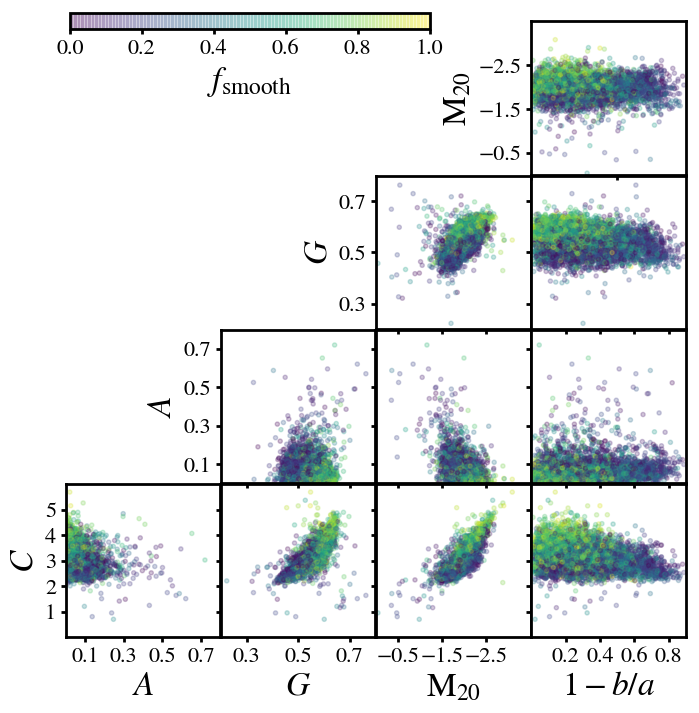
\includegraphics[width=5in]{Figures/morph_params_random_sample_fsmooth_colored_clean.png}
\caption[Automated morphologies as a function of Galaxy Zoo 2 \fsmooth]{Here a random sample of 5000 galaxies are plotted in every possible planar combination of our morphology structural indicators where the color denotes the galaxy's debiased \fsmooth~fraction from GZ2. As expected, galaxies with higher \fsmooth~are found in locations where early-types are typically seen: notably they have larger $C$ and $G$, and smaller \M{20}.}
\label{fig: morphs as a fcn of fsmooth}
\end{figure}


%Gini coefficient sucks \citep{Lisker2008}.


\begin{figure}
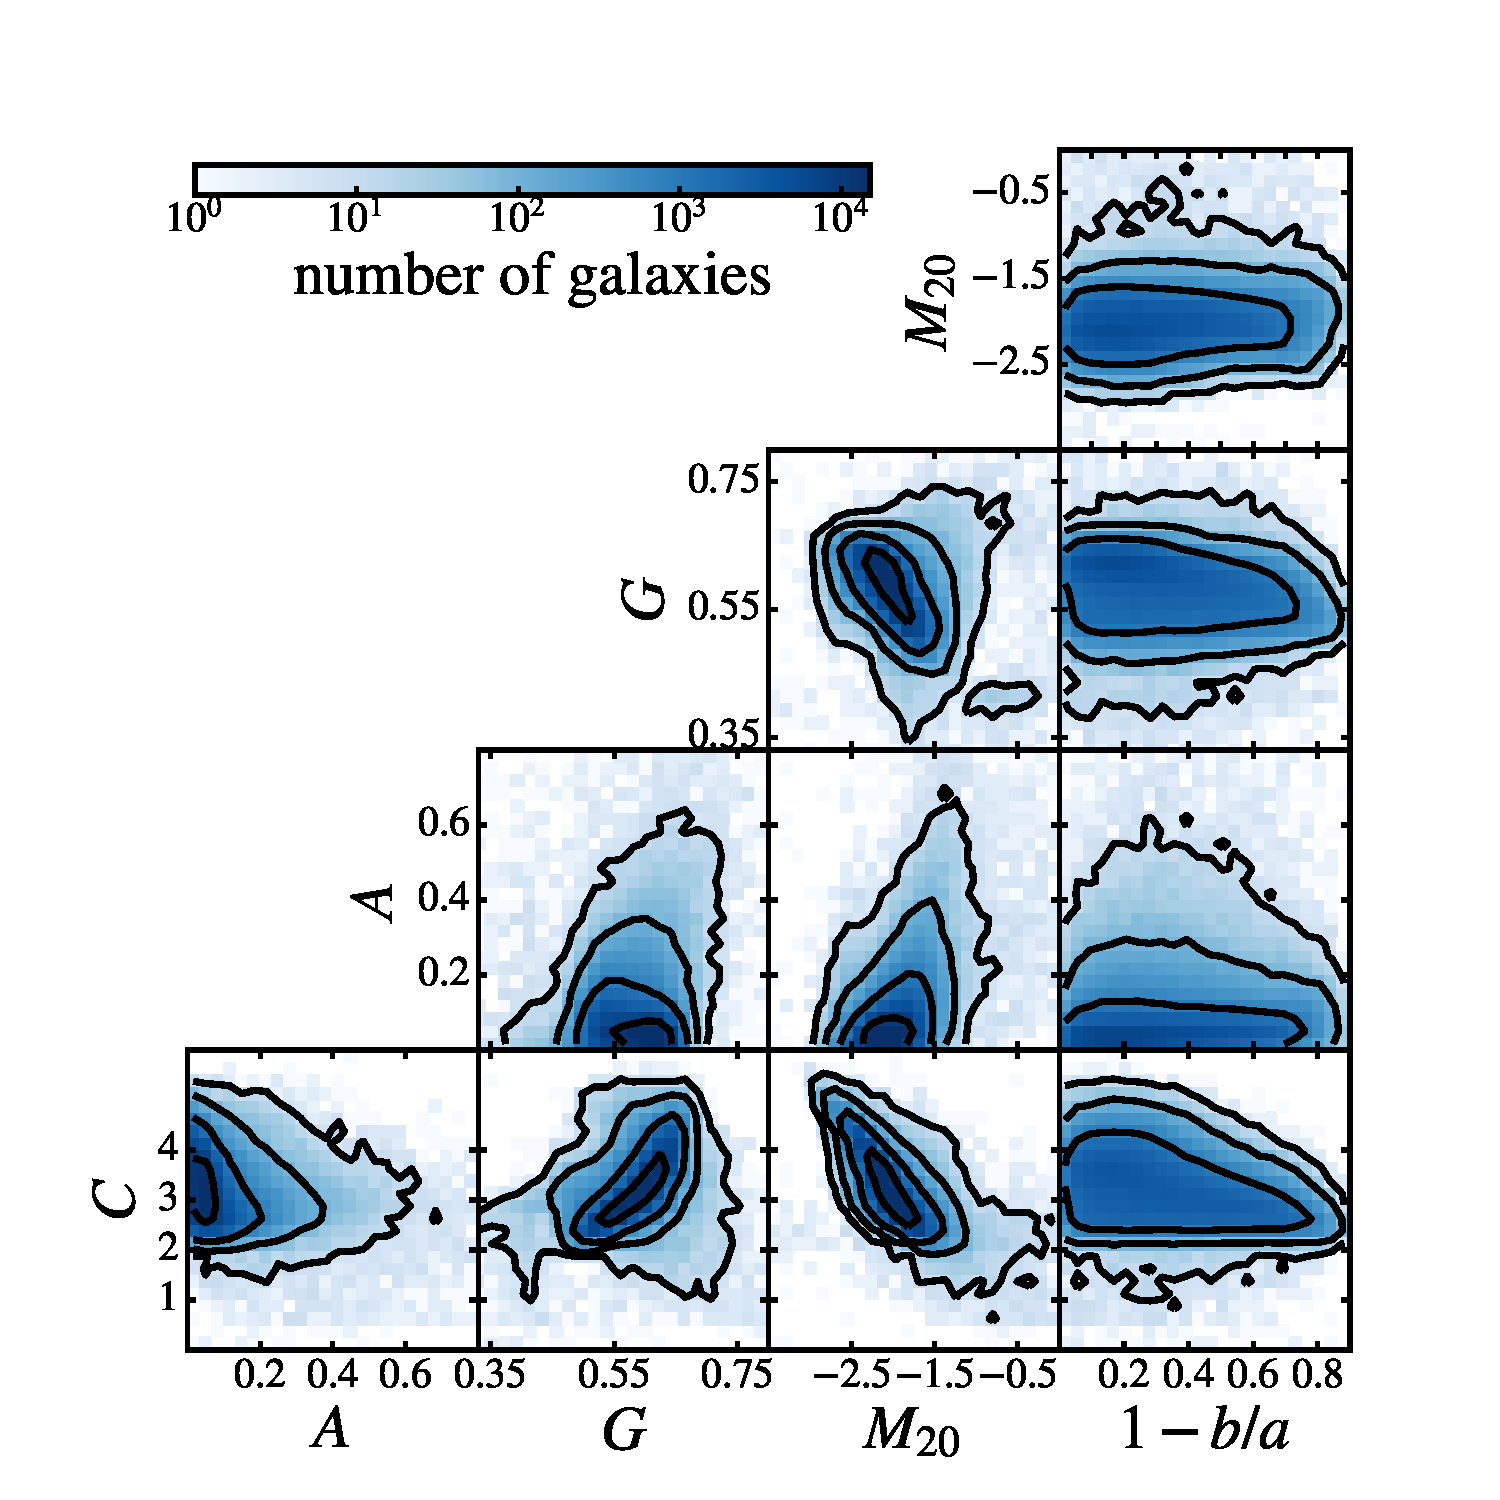
\includegraphics[width=\textwidth]{Figures/human_machine/A2b.pdf}
\caption[Automated morphologies for the full GZ2 sample.]{\textit{Right.} Relation between measured morphology diagnostics for more than 280K SDSS galaxies. Correlations between several diagnostics are immediately obvious and not all relations are likely to be linear. These points will be revisited in Chapter \ref{chap:4} when we discuss machine learning algorithms.}
\label{fig: morphs}
\end{figure}



\section{Catalog of morphological indicators for 282350 SDSS galaxies}
Put in a big table here with a subsample of the catalog? Link to somewhere online where the rest of the catalog can be found? 


\begin{deluxetable}{lccccccccc}
\rotate
\tablecolumns{10}
\tablewidth{0pt}
\tablecaption{Morphology Diagnostics for $\sim$283K SDSS Galaxies in the GZ2 Sample}
\tablehead{
	\colhead{DR7 objID} &
	\colhead{RA}		&
	\colhead{DEC}		&
	\colhead{R$_p$}		&
	\colhead{$C$}		&
	\colhead{$A$}		&
	\colhead{\M{20}}	&
	\colhead{$G$}		&
	\colhead{e}			&
	\colhead{flags}		
}
\startdata
587722981736054938 & 170.749 &	-1.25746 &	44.09 & 2.556 & 0.0243 & -1.888 & 0.539 & 4.289 &	\\
\enddata
\end{deluxetable}